%\documentclass[12pt,twoside]{article}
%\usepackage[inner=1in,outer=0.6in,top=0.7in,bottom=1in]{geometry}
%\usepackage{xeCJK}
%\setmainfont{Times New Roman}
%\setsansfont{Verdana}
%\setmonofont{Courier New}                    % tt
%\setCJKmainfont{微軟正黑體}
%\setCJKfamilyfont{kai}{標楷體}		% for changing the title font in title.pgf -> have to manually 
%\usepackage{graphicx}
%\usepackage{pgf}
%\usepackage{pstricks,pst-node}
%
%\renewcommand{\today}{西元\number \year 年\ifcase \month \or 1月\or 2月\or 3月\or 4月\or 5月\or 6月\or 7月\or 8月\or 9月\or 10月\or 11月\or 12月\fi
%} 
%
%\begin{document}

\noindent\begin{pspicture}(-0.4in,0in)(6.5in,8cm)
%\psgrid[unit=.5in]

\rput[br](6.5in,-0.2cm){
\rnode{name}{\large 東寧軟咖
}}

\rput[br](6.5in,0.6cm){
\rnode{time}{\large \today
}}

\rput[bl](-0.5in,2.6cm){
\rnode{logo}{\includegraphics[scale=0.37]{./figs/logo_June27_2016.png}
%\includegraphics[scale=0.37]{../../figs/logo_June27_2016.png}
}}

\rput[bl](-0.44in,6.4cm){
\rnode{title}{\resizebox{6.9in}{!}{\Huge 陀螺,\hspace{0.8cm}方向追蹤,與計算機轉動模擬器}
%從陀螺聊到姿態追蹤與\\
%物理模擬引擎
%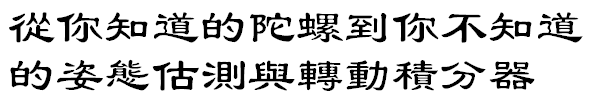
\includegraphics[scale=0.6]{./otherstuff/gyro_title_line4.PNG}%./otherstuff/
}}
%\psline(-0.8cm,0.4cm)(12.3cm,0.4cm)
\psline[linewidth=0.2cm](-0.4in,2.8cm)(6.5in,2.8cm)

\rput[br](6.5in,2cm){
\rnode{running_title1}{\large \textcolor{gray}{從基礎的牛頓尤拉方程與貼體角速度應用到姿態追蹤}
}}

\rput[br](6.5in,1.4cm){
\rnode{running_title2}{\large \textcolor{gray}{與電腦的轉動積分器,實作與應用}
}}



\rput[br](6.5in,3.3cm){
\rnode{website}{whymrandersonwhy.pythonanywhere.com
}}

\rput[br](6.5in,3.8cm){
\rnode{gss}{\Large \textcolor{gray}{GyroSoft Simulation}
}}

%\rput[B](5.5 cm,3.3cm){
%\rnode{E}{
%%\includegraphics[scale=0.5]{./decoration_line.PNG}
%\includegraphics[scale=0.5]{./otherstuff/decoration_line.PNG}
%}}





\end{pspicture}


%\end{document}